
\subsection{Basic transformations}

The basic transformations that are supported include
translation, rotation and scaling along the x-axis
and the y-axis. The order of transformation is
origin, scaling, rotation, translation.

Transformations are controlled through the CollisionInfo
data type.

It should be noted that some transformations make
collision objects uncollidable. These cases include
when either scaling factor is 0. In these cases,
the object causes no collision. The reason is that
such a scaling factor does not make a lot of sense,
because the object in question would have zero width/height.

As an example of basic transformations, consider a 4-by-4 rectangle
with an origo in the corner marked by the blue cross.
A transformation by translation P(0, 2), rotation 30 degrees
(in the library, it would be $\pi / 6$ radians), scale-x = 1.5
and scale-y = 0.5.

The initial mask is shown in figure \ref{fig:before_transformation},
while the result of the transformation is shown in figure \ref{fig:after_transformation}.

\begin{figure}[p]
	\centering
	\begin{subfigure}[b]{0.3\textwidth}
	  \centering
	  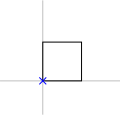
\includegraphics{transformations/before_transformation.pdf}
	  \subcaption{Before transformation}
	  \label{fig:before_transformation}
	\end{subfigure}
	\begin{subfigure}[b]{0.3\textwidth}
	  \centering
	  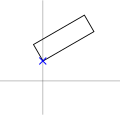
\includegraphics{transformations/after_transformation.pdf}
	  \subcaption{After transformation}
	  \label{fig:after_transformation}
	\end{subfigure}
\caption{Transformation, before and after}
\label{fig:transformation}
\end{figure}

In the implementation of the engine, transformations are done by
a 3-by-3 matrix, even though the coordinates are only 2-dimensional.
The reason is that working with a single matrix for transformations
and inverse transformations is simple and fast.
If only scaling and transformation was supported,
a 2-by-2 matrix would be sufficient. But since translation is
also supported, a 3-by-3 matrix is needed.
The reason is the same as to why 4-by-4 matrices are used in
3D graphics, even though only 3 dimensions are used.
See also \url{http://en.wikipedia.org/wiki/Homogeneous_coordinates#Use_in_computer_graphics}.

